\section{Conclusion}

% Time and frequency domains
\subsection{Time and frequency domains}
The first thing we can observe when comparing the time and frequency controllers is that we do not have a \textbf{static error} in the frequency domain, thanks to the lag compensator. The \textbf{noise rejection} is quite good in both domains. In the time one, it may be explained by the fact that the observer acts as a filter. Indeed, the output of the system being one of the states it has to approximate on the basis of two non noisy inputs and a noisy one, the noise rejection is simplified. For the frequency domain, it is done thanks to the low-pass filter.\par
Concerning the reaction to a \textbf{reference change}, we found out that the frequency controller allowed us to reach that reference before $3s$, at the cost of an unbelievably high force applied on the damper. It is not plotted because we ran out of space and it was not asked explicitly, but we have a spike at $1.3m$ for the displacement of the building then a stabilization at 1m. It is not the case for the time domain, where we have huge displacements and no stabilization that we can observe in a reasonable time. That is counter-intuitive as we thought that a controller in time domain would track a reference better than one in frequency domain.\par
Concerning the \textbf{delays}, the frequency domain deals with them more easily than the time domain, although not by much. Indeed, as can be seen in Figure \ref{fig:delay}, the time controller is also quite good with small delays ($0.02s$).
\begin{figure}[H]
    \centering
    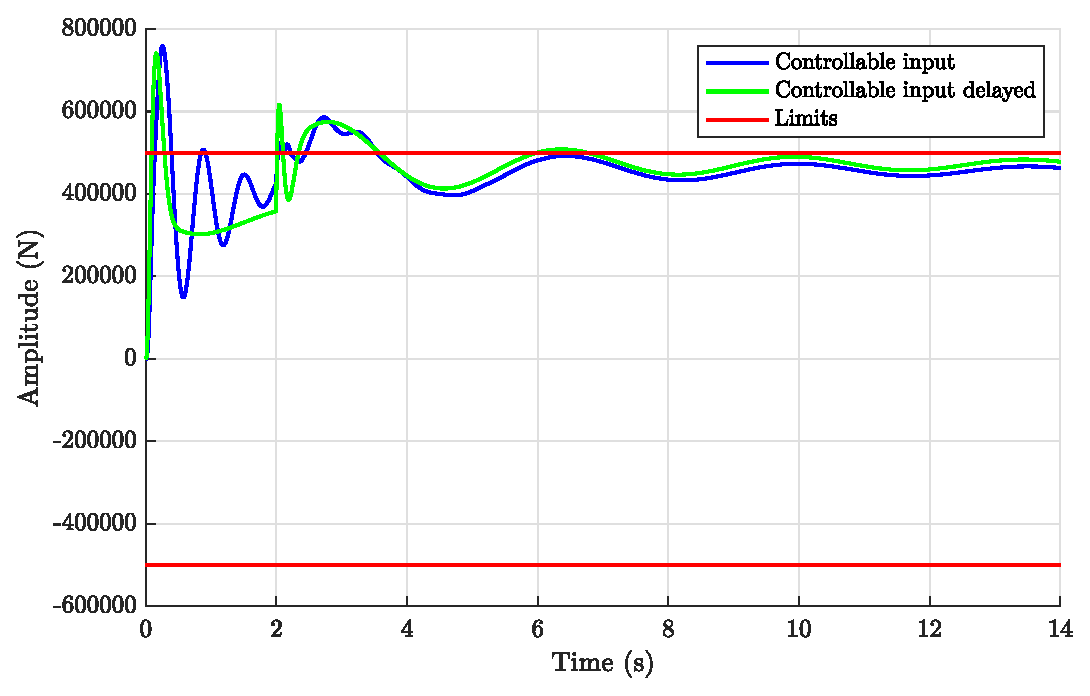
\includegraphics[scale = 0.7]{resources/eps/3_delay-controllable-input.eps}
    \caption{Time controller simulation with 0.02s of delay.}
    \label{fig:delay}
\end{figure}

% General conclusion
\subsection{General conclusion}
This project allowed us to put in practice a lot of concepts that were explained in the theoretical lectures. However, we could not reach controllers that complied with the constraints Pr Denoël gave us (an acceleration between $0.3$ and $0.6g$). This may come from the fact that some parameters had wrong values or that we oversimplified the problem.\par
We played with the different parameters of our controllers a huge amount of time in order to reach these constraints and the results presented in this report are the best we could manage. Using a bigger mass for the damper would have helped us reach our constraints, but we felt like $30$ tons was already very heavy. We have thus decided to use an acceleration that was high, but not completely out of touch with reality. Although our results are not perfectly aligned with our initial constraint, we feel like we have understood the theoretical concepts we have applied, which was ultimately the goal of this project.
